\documentclass{article}

\usepackage{amsmath}
\usepackage{amssymb}
\usepackage{tikz}
\usetikzlibrary{automata,positioning,arrows}
\tikzset{
	>=stealth',
	initial text=$ $
	}

\title{Assignment 4}
\date{2019-02-07}
\author{MONTGOMERY, BENNET 20074049 CISC223\\
		\and DALLAS, SPENCER 20048480 CISC223\\
		\and GOEL, CHRISTOPHER 20053408 CISC223\\
		\and VIOLO, JARED 20051382 CISC223}

\begin{document}
	\maketitle
	\section*{Q1.}
	The sets $F$ and $Q - F$ for this DFA where $F$ is the set of accepting states and $Q - F$ is the set of states that are not accepting states are $F = \{B, C\}$ and $Q - F = \{A, D\}$. Recall that all state pairs $(q_1, q_2)$ are marked before the first minimization step where $q_1 \in F$ and $q_2 \in Q - F$, therefore the following state pairs are marked initially:
		\begin{align*}
			&(A, B)\\
			&(A, C)\\
			&(D, C)\\
			&(D, B)
		\end{align*}
	and the following state pairs are unmarked initially:
		\begin{align*}
			&(A, D)\\
			&(B, C)
		\end{align*}
	In the first step of minimization, we apply the transition function $\delta$ to the members of each unmarked state pair and $\forall x \in \Sigma$:
		\begin{align*}
			(\delta(A, a), \delta(D, a)) &= (B, B)\\
			(\delta(A, b), \delta(D, b)) &= (C, C)\\
			(\delta(B, a), \delta(C, a)) &= (D, C)\\
			(\delta(B, b), \delta(C, b)) &= (B, C)
		\end{align*}
	Since applying $\delta$ to $(B,C)$ with the parameter $a$ yielded $(D,C)$, a state pair that has already been marked, the state pair $(B, C)$ is marked at the end of the first step. In the second minimization step, we apply $\delta$ to the only remaining unmarked state pair:
		\begin{align*}
			(\delta(A, a), \delta(D, a)) &= (B, B)\\
			(\delta(A, b), \delta(D, b)) &= (C, C)
		\end{align*}
	Neither $(B,B)$ nor $(C,C)$ are previously marked state pairs, so $(A, D)$ remain unmarked. Since we only have unmarked state pairs remaining at the end of step 2, we are now finished the minimization process. We have determined that the states $A$ and $D$ are indistinguishable (as the only remaining unmarked state pair), so we merge them in the resulting DFA:
		\begin{figure}[!h]
			\centering
			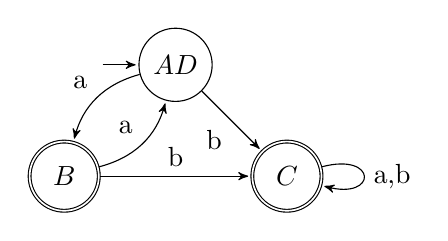
\begin{tikzpicture}[shorten >=1pt,node distance=2cm,on grid,auto]
				\node[state,initial](AD){$AD$};
				\node[state,accepting] (B) [below left=of AD] {$B$};
				\node[state,accepting] (C) [below right=of AD] {$C$};
				\path[->]
				(AD) edge [bend right] node [swap] {a} (B)
					edge node [swap] {b} (C)
				(B) edge [bend right] node {a} (AD)
					edge node {b} (C)
				(C) edge [loop right] node {a,b} ();
			\end{tikzpicture}
		\end{figure}
	
	\section*{Q2.}
	\subsection*{(a)}
		This language is generated by a context free grammar for this alphabet where $V = \{S, X, Y\}$ and $P$ is the following production set:
		\begin{align*}
			S &\rightarrow aXbb \hphantom{a} | \hphantom{a} cccYd\\
			X &\rightarrow aXbb \hphantom{a} | \hphantom{a} \epsilon\\
			Y &\rightarrow cccYd \hphantom{a} | \hphantom{a} \epsilon
		\end{align*}
	The string $c^9d^3$ is generated with the derivation $S \Rightarrow cccYd \Rightarrow ccccccYdd \Rightarrow cccccccccYddd \Rightarrow cccccccccddd$.
	\subsection*{(b)}
	This language is generated by a context free grammar for this alphabet where $V = \{S, X, Y\}$ and $P$ is the following production set:
		\begin{align*}
			S &\rightarrow aXbbcccYd\\
			X &\rightarrow aXbb \hphantom{a} | \hphantom{a} \epsilon\\
			Y &\rightarrow cccYd \hphantom{a} | \hphantom{a} \epsilon
		\end{align*}
	The string $a^2b^4c^9d^3$ is generated with the derivation $S \Rightarrow aXbbcccYd \Rightarrow aaXbbbbccccccYdd \Rightarrow aabbbbcccccccccYddd \Rightarrow aabbbbcccccccccddd$
	\subsection*{(c)}
	This language is generated by a context free grammar for this alphabet where $V = \{S, X\}$ and $P$ is the following production set:
		\begin{align*}
			S &\rightarrow aSd \hphantom{a} | \hphantom{a} abbXcccd\\
			X &\rightarrow bbXccc \hphantom{a} | \hphantom{a} \epsilon
		\end{align*}
	The string $a^2b^2c^3d^2$ is generated with the derivation $S \Rightarrow aSd \Rightarrow aabbXcccdd \Rightarrow aabbcccdd$
	\subsection*{(d)}
	This language is generated by a context free grammar for this alphabet where $V = \{S, W, X, Y, Z\}$ and $P$ is the following production set:
		\begin{align*}
			S &\rightarrow aaabWc \hphantom{a} | \hphantom{a} aaXc \hphantom{a} | \hphantom{a} bbcYdd \hphantom{a} | \hphantom{a} bbZ\\
			W &\rightarrow bW \hphantom{a} | \hphantom{a} \epsilon\\
			X &\rightarrow aaabWc \hphantom{a} | \hphantom{a} aaXc\\
			Y &\rightarrow cYdd \hphantom{a} | \hphantom{a} \epsilon\\
			Z &\rightarrow bbcYdd \hphantom{a} | \hphantom{a} bbZ
		\end{align*}
	The string $b^2c^2d^4$ is generated with the derivation $S \Rightarrow bbcYdd \Rightarrow bbccYdddd \Rightarrow bbccYdddd \Rightarrow bbccdddd$.
\end{document}